%----------------------------------------------------------------------------------------
%    PACKAGES AND THEMES
%----------------------------------------------------------------------------------------

\documentclass[aspectratio=169,xcolor=dvipsnames]{beamer}
\usetheme{SimplePlus}

\usepackage{hyperref}
\usepackage{graphicx} % Allows including images
\usepackage{booktabs} % Allows the use of \toprule, \midrule and \bottomrule in tables

%----------------------------------------------------------------------------------------
%    TITLE PAGE
%----------------------------------------------------------------------------------------

\title{Nobel Ontology}
\subtitle{Group A3D}

\author{Andrea Bruttomesso, Alessandro Corr\`o, Davide Seghetto, Andrea Stocco}

%\institute
%{
%    Department of Computer Science and Information Engineering \\
%    National Taiwan University % Your institution for the title page
%}
\date{\today} % Date, can be changed to a custom date

%----------------------------------------------------------------------------------------
%    PRESENTATION SLIDES
%----------------------------------------------------------------------------------------

\begin{document}

\begin{frame}
	% Print the title page as the first slide
	\titlepage
\end{frame}

\begin{frame}{Overview}
	% Throughout your presentation, if you choose to use \section{} and \subsection{} commands, these will automatically be printed on this slide as an overview of your presentation
	\tableofcontents
\end{frame}

\section{Domain of Interest}

\begin{frame}{Domain of Interest}
	We have chosen the domain of scientific research. Specifically, we aim to analyze potential correlations among Nobel Prize winners,
	their publications, and the research funding invested by various countries. This domain was selected because it allows us to reveal potential historical
	and geographical patterns in scientific research.
\end{frame}

%------------------------------------------------
\section{Ontology Design}
%------------------------------------------------

\begin{frame}{Nobel Ontology}
	\begin{figure}
		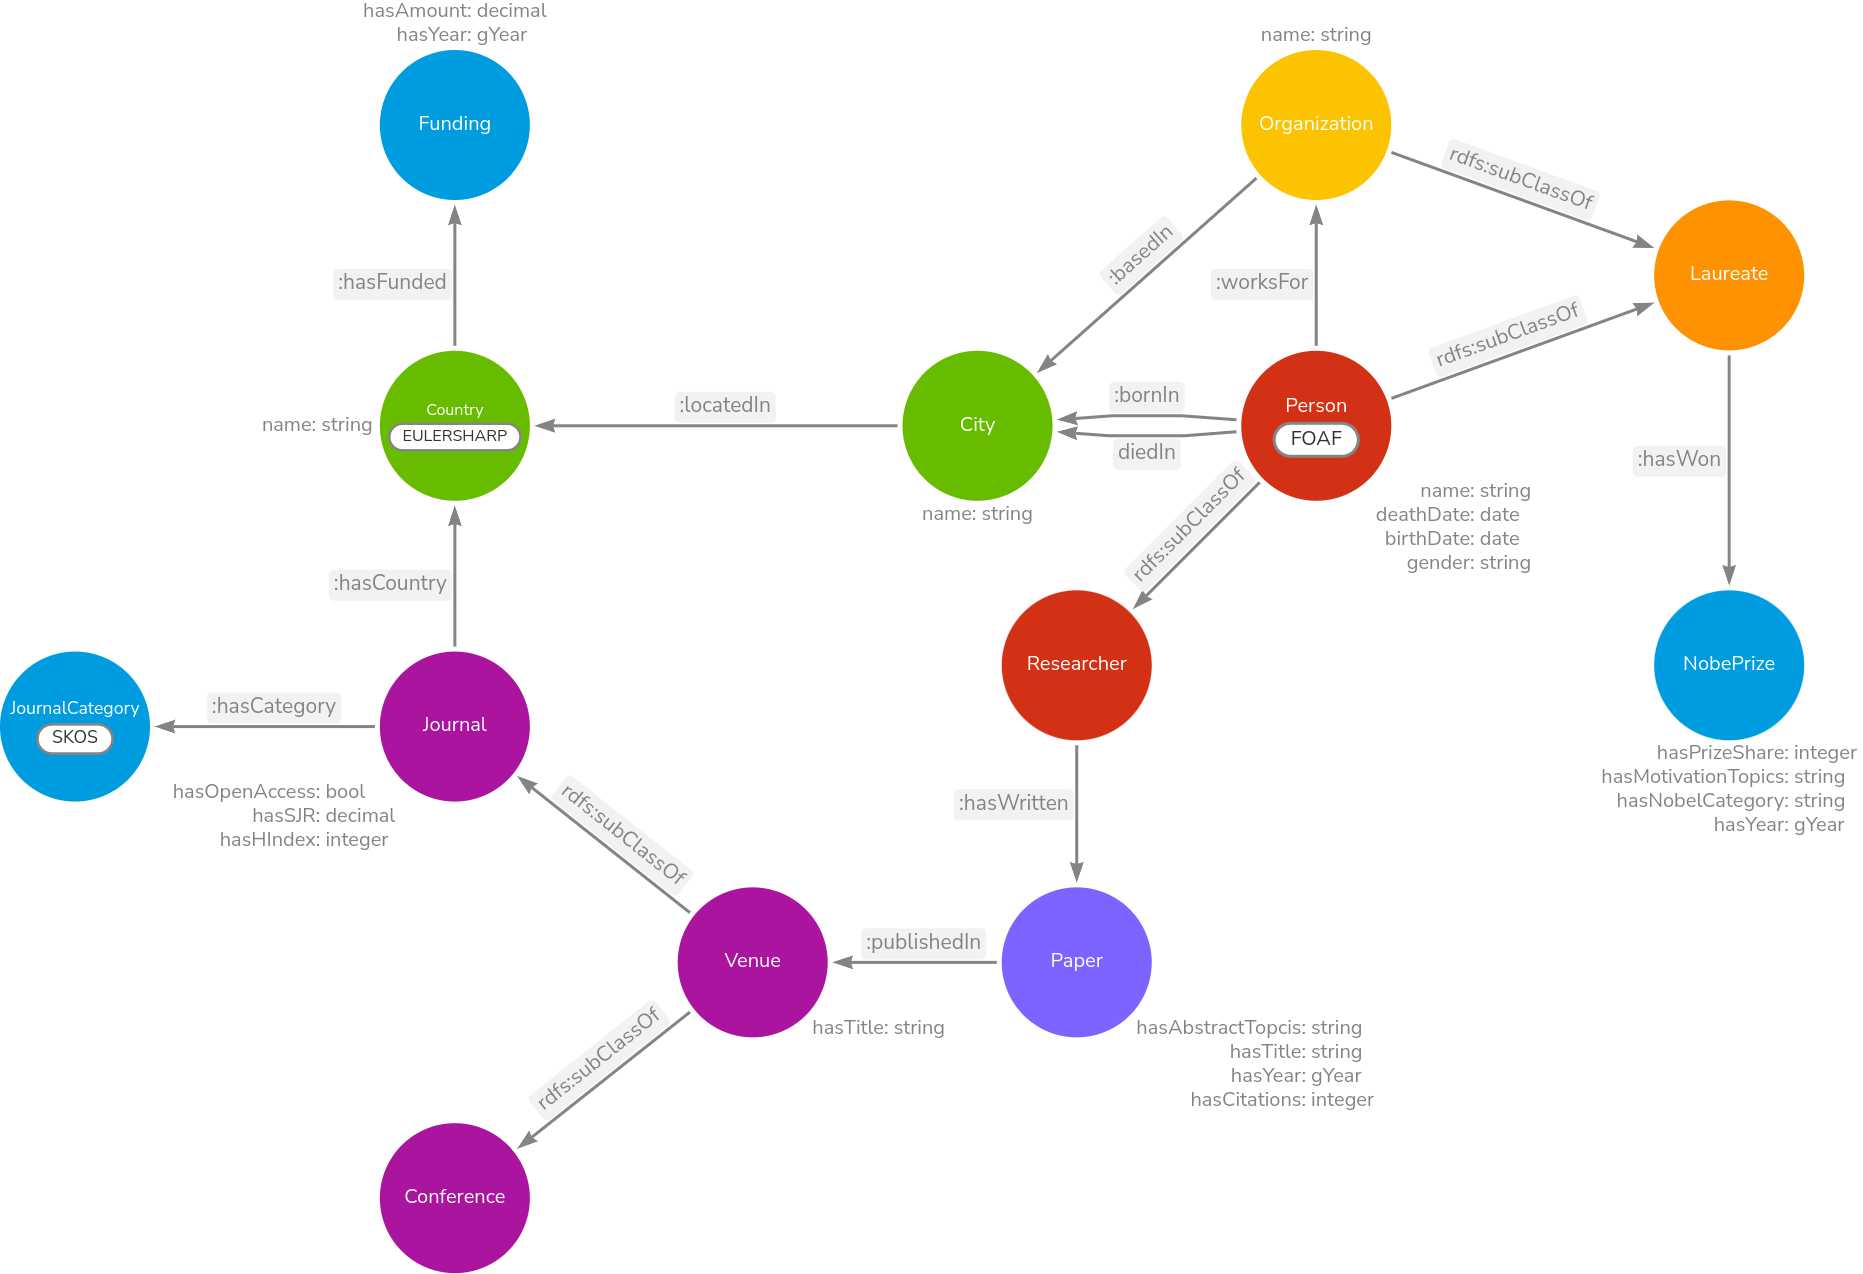
\includegraphics[width=0.75\linewidth]{../nobelOntologyTransparent.png}
	\end{figure}
\end{frame}

\section{Problems}

\begin{frame}{Problems}
	\begin{itemize}
		\item Prize share
		\item Used only a portion of the papers dataset
	\end{itemize}
\end{frame}

%------------------------------------------------

\begin{frame}{Blocks of Highlighted Text}
	In this slide, some important text will be \alert{highlighted} because it's important. Please, don't abuse it.

	\begin{block}{Block}
		Sample text
	\end{block}

	\begin{alertblock}{Alertblock}
		Sample text in red box
	\end{alertblock}

	\begin{examples}
		Sample text in green box. The title of the block is ``Examples".
	\end{examples}
\end{frame}

%------------------------------------------------

\begin{frame}{Multiple Columns}
	\begin{columns}[c] % The "c" option specifies centered vertical alignment while the "t" option is used for top vertical alignment

		\column{.45\textwidth} % Left column and width
		\textbf{Heading}
		\begin{enumerate}
			\item Statement
			\item Explanation
			\item Example
		\end{enumerate}

		\column{.45\textwidth} % Right column and width
		Lorem ipsum dolor sit amet, consectetur adipiscing elit. Integer lectus nisl, ultricies in feugiat rutrum, porttitor sit amet augue. Aliquam ut tortor mauris. Sed volutpat ante purus, quis accumsan dolor.

	\end{columns}
\end{frame}

%------------------------------------------------
\section{Analytics}
%------------------------------------------------

\begin{frame}{Query 1}
	\begin{table}
		\begin{tabular}{l l l}
			\toprule
			\textbf{Treatments} & \textbf{Response 1} & \textbf{Response 2} \\
			\midrule
			Treatment 1         & 0.0003262           & 0.562               \\
			Treatment 2         & 0.0015681           & 0.910               \\
			Treatment 3         & 0.0009271           & 0.296               \\
			\bottomrule
		\end{tabular}
		\caption{Table caption}
	\end{table}
\end{frame}

%------------------------------------------------

\begin{frame}{Query 2}
	\begin{theorem}[Mass--energy equivalence]
		$E = mc^2$
	\end{theorem}
\end{frame}

%------------------------------------------------

\begin{frame}{Query 3}
	Uncomment the code on this slide to include your own image from the same directory as the template .TeX file.
	%\begin{figure}
	%\includegraphics[width=0.8\linewidth]{test}
	%\end{figure}
\end{frame}

%------------------------------------------------

\begin{frame}
	\Huge{\centerline{\textbf{Questions?}}}
\end{frame}

%----------------------------------------------------------------------------------------

\end{document}
